\subsection{Firestorage}

Visto que a desenvolvedora do \textit{Flutter} e do \textit{Firebase} é a mesma, esta disponibilizou recursos que facilitam a utilização desta ferramenta pelo \textit{Flutter}, sendo assim todas as imagens e vídeos de utilizadores, publicações e comentários são guardadas diretamente da aplicação para o \textit{firestorage}, assim como o acesso às mesmas é realizado diretamente.

Para permitir este tipo de acesso o \textit{Firebase} disponibiliza de uma ferramenta que permite através do terminal configurar a ligação entre o projeto e o servidor do \textit{Firebase}, sendo que no final apenas é necessário importar a biblioteca do serviço do \textit{Firebase} que se deseja e invocar a classe do mesmo para realizar alguma ação.

Os ficheiros são então organizados conforme o seu contexto. Para utilizadores existe a pasta utilizadores, para tópicos existe a pasto tópicos e para comentários existe a pasta comentários. 


A pasta utilizadores, como cada utilizador, apenas contém uma imagem, então estas são guardas com o nome do id do utilizador e na eventualidade de já existir é substituída. No caso de tópicos e comentários como podem conter várias imagens e vídeos, então estes são guardados em pastas com os ficheiros referentes e que têm por nome os ids dos tópicos ou comentários.

\begin{figure}[htb]%
  \centering
  \subfloat[\centering Raiz do firestorage]{{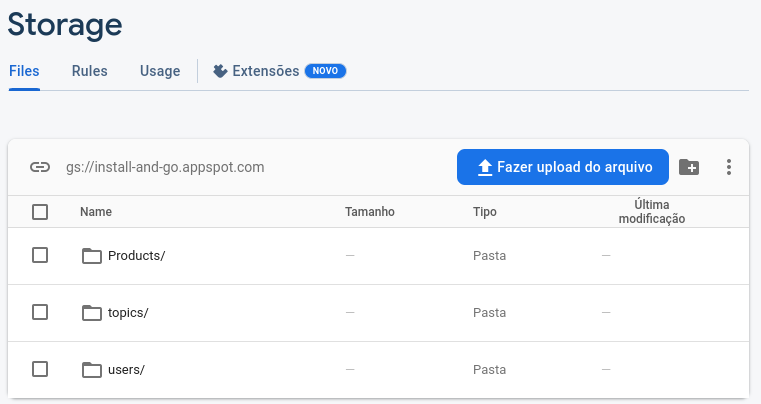
\includegraphics[width=0.7\textwidth]{images/implementacao/frontend/firestorage/all.png} }}%
  \qquad
  \subfloat[\centering Pasta topics do firestorage]{{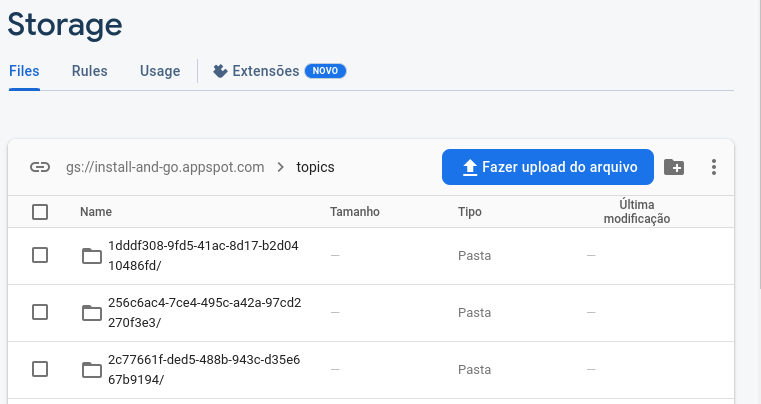
\includegraphics[width=0.7\textwidth]{images/implementacao/frontend/firestorage/topics.png} }}%
  \label{fig:76}%
\end{figure}